\documentclass{aa}
% \documentclass[referee]{aa}
% \documentclass[bibyear]{aa} 
\usepackage[varg]{txfonts}
\bibpunct{(}{)}{;}{a}{}{,}
\usepackage{graphicx}
\usepackage[noend]{algpseudocode}
\usepackage{cellspace}
\usepackage{url}
\usepackage{color}
\usepackage[toc, page]{appendix}
\usepackage[utf8]{inputenc} %unicode support

\def\simon#1{{\bf {\color{green}[#1 -- Simon]}}}
\def\Simon#1{{\bf {\color{green}[#1 -- Simon]}}}

\begin{document}
\title{On the identification of Earth-impacting asteroids using an artificial neural network}
\author{John D. Hefele\inst{1}
\and Francesco Bortolussi\inst{2}
\and Simon Portegies Zwart\inst{3}}
\institute{Sterrewacht, Leiden University, Leiden, NL
\and LIACS, Leiden University, Leiden, NL
\and Sterrewacht, Leiden University, Leiden, NL}
\date{Received DD MM YYYY / Accepted DD MM YYYY}

\abstract{ We identify potentially Earth impacting asteroids by means
  of an artificial neural network. We name the resulting instrument
  the Hazardous Object Identifier (or HOI for short). The network is
  trained on an artificial set of known impactors which was generated
  by launching $10^5$ test particles over a future period of 20,000
  years from the Earth's surface and integrating them with a
  symplectic integrator backwards in time to todays date.  The
  integrations, forwards as well as backwards in time, included all
  known planets of the Solar System.  The neural network was
  subsequently trained on the orbital evolution of these known
  impactors.  HOI was able to positively identify 95.25\% of the
  simulated known-impactors among an ensamble of known non-impactors.
  The same network correctly classified 90.99\% of the potentially
  hazardous objects identified by NASA without prior trained, and
  99.9\% of the objects that approached Earth within 0.05\,au in the
  next millennium.  }

\keywords{Comets: general -
  Minor planets, asteroids: general - Methods: data analysis -
  Methods: statistical}

\titlerunning{On the identification of
  Earth-impacting asteroids using an artificial neural network}

\authorrunning{J. D. Hefele et al.}
\maketitle


\section{Introduction}
\label{SEC:Introduction}

In 1990, the US Congress requested for NASA to establish two workshops
to focus on the identification of potentially hazardous objects 
\footnote{Hereafter PHOs. Objects with a maximum orbit intersection
  distance from Earth of 0.05\,au and brighter than an absolute
  magnitude of 22.0 \citep{NasaPHA}.}  and on methods to alter their
orbits to prevent an impact \citep{milani2002}. The workshops led to
the establishment of the \textit{Sentry: Earth Impact Monitoring}
system \citep{Sentry}.  If a hazardous asteroid would be identified
sufficiently early before impact, it would be possible to mitigate the
impact by means of an appropriate space mission to alter the
asteroid's orbit through a gravitational tugboat
\citep{10.2307/26060526}, or by obliterating it with a nuclear warhead
\citep{BARBEE201837}.  Both mitigation strategies require years of
preparation, which makes the early detection of hazardous objects
vital to allow ample time for mission preparation.

The Sentry system adopts a Monte Carlo approach in which millions of
virtual objects are launched with orbital parameters statistically
sampled from within the error ellipsoid of the observed asteroids. The
impact probability is subsequently determined on the fraction of
virtual asteroids that reach Earth within some pre-determined striking
distance \citep{milani2002}, typically 0.05\,au. In this approach, the
orbits of many asteroids are integrated numerically and the final
parameter space is considered to represent the probability-density
distribution of the respective objects. The calculation of this
probability density distribution relies on the algorithm and
implementation used to integrate the orbits of the asteroids.  The
time scale over which such integrations remains reliable depends on
the degree by which the asteroid's orbit is chaotic, i.e. on the value
of the largest positive Lyapunov exponent.
Additionally, the
reliability of such computations depends on the ability of the
integrator to obtain a solution, such that the integration complies to
the concept of {\em nagh Hoch}\footnote{\textbf{\textit{Nagh Hoch} is
    the concept that an ensemble of random initial realizations in a
    wide range of parameters gives statistically the same result as
    the converged solutions of the same ensemble realizations.}}
\citep{PORTEGIESZWART2018160}.

Both of these concepts are not guaranteed with the adopted numerical
schemes, and the results reach questionable proportions as soon as the
asteroid experiences a close encounter with any object other than the
Earth. In the latter case, the phase space of possible solutions grows
exponentially due to the chaotic nature of the equations of motion.
Establishing the chaotic nature of an asteroid is limited by the
accuracy of its orbital determination. This is generally realized by
observing any particular asteroid a number of times. These
observations result in a data arc, the fraction of the orbit over
which the object was observed.  The adopted Monte-Carlo method used in
the Sentry system is expected to be reliable for at most a few dozens
of years \citep{HorizonsManual} for asteroids for which the observed
data arc is smaller than a month, which is 12.9\% of all small-bodies
\citep{dastcom5}.

Considering the high degree of chaotic motion (small Lyapunov time
scale) in asteroids and the consequential exponential divergence of
their orbits, one can wonder if it is worth the effort to perform
extensive computer simulations in order to track the orbital
trajectories of a large number of particles so long as the veracity of
the orbital integration can not be guaranteed. For the most chaotic
asteroids, the impact probability sensitively depends on the
statistics because these objects snap the largest volume in phase
space. It is therefore essential to adopt a more course grained method
that is able to classify potential impactors based on fewer and less
reliable data.  Such a method would free-up computer time that can
subsequently be used to produce more reliable impact probabilities for
the most promising candidate impctors using the method adopted in the
Sentry system.

We explore the population of asteroids, and in particular the
potentially dangerous ones, by means of automatic machine recognition
through a combination of numerical integrations and a trained neural
network similar to the architectures described in \citep{ref1} and
\citep{ref2}, which were used for classifying hazardous taxonomy and
solar sail transfer time estimation. It is a statistical approach in
which we determine the prospect for impact of the known population of
asteroids gathered from the \textit{dastcom5} off-line database
\citep{dastcom5}.  Our analysis is mediated by an artificial
neural-network dubbed HOI\footnote{This also means ``Hello'' in the
  Dutch language.} for ``Hazardous Object Identifier'', which was
trained on a population of known-impactors (KI) and a random sample
from the observed database.  The network was implemented and trained
using the \textit{TensorFlow framework} \citep{TensorFlow}. The $10^5$
KIs are machine generated from a population of asteroids that start
their orbit on a random position of Earth's surface and are launched
radially away with the planet's escape speed. The orbits of impacting
asteroids and planets in orbit around the Sun was performed using the
\textit{Huayno} integrator \cite{2014A&A...570A..20J} in the
Astrophysical Multipurpose Software Environment
\cite{2018araa.book.....P}.  These objects are subsequently integrated
backwards in time together with the planets in the Solar system for up
to 20,000 years. To train HOI, these computer generated KIs are then
mixed with an equal number of observed asteroids, which we assume to
be non-impacting.  The trained network is then used on another random
selection of observed asteroids in order to identify potential
impactors (PIs). All the objects that were not identified by the model
as PIs, and that were not initially labeled as KIs, are referred to as
unidentified objects (UOs).

We begin by describing HOI's architecture in
section\,\ref{SEC:1D_CNN}, which is followed by a discussion of the
generation of the small-body datasets in section\,\ref{SEC:Data}. The
results are examined in section\,\ref{SEC:Results} and conclusions are
drawn in section\,\ref{SEC:Conclusions}. All the code used to train
the neural network, generate data, and evaluate the results are
publicly available on \textbf{GitHub}\footnote{
  \url{https://github.com/mrteetoe/HOI}}.
%\citep{koon,oreg,khar,zvai,xjon,schn,pond,smith,marg,hunn,advi,koha,mouse}

\section{HOI's architecture}
\label{SEC:1D_CNN}

Neural networks are well suited for recognizing complex patterns
hidden in multi-dimensional data-sets. In our particular case, we
strive to identify observed objects that have topologically similar
trajectories to the trajectories of the population of known
impactors. Because we are no longer reliant on calculations that
attempt to estimate the asteroids position at a particular point in
time, the network is more resilient to perturbations of the initial
conditions i.e. chaotic motion.

The problem reduces to a discrete binary classification task, where
the two mutually exclusive classes are either ``potential impactors''
(PIs) or ``unidentified objects'' (UOs). For the purpose of our
experiments, the UOs are what we would consider ``benign objects'',
i.e. objects that are not regarded as PIs. To quantify the network's
accuracy, the standard ``cross entropy'' cost function is used, which
we define as:
\begin{equation}
	\label{cost_function}
	H(y,\hat{y})=-\sum_i^{N} y_i \text{ln}(\hat{y}_i)+(1-y_i)\text{ln}(1-\hat{y}_i).
\end{equation}
Here $y$ is the actual value, or label, $\hat{y}$ is the predicted
value, and $N$ is the total amount of predictions. This cost function
has the convenient property that its derivative with respect to some
input weight, $w$, scales linearly with the difference between the
label and predicted value \citep{Nielson}:
\begin{equation}
	\frac{\partial C}{\partial w}=\frac{1}{N}\sum^{N}_i x(\hat{y}_i-y_i).
\end{equation}
Here $x$ is the input value by which $w$ is multiplied.

To minimize (\ref{cost_function}), the ``Adam Optimizer'' is used,
which expands upon na\"{i}ve stochastic gradient descent by adapting
its learning rate based on both the average of the first and second
moments of the gradients \citep{AdamOptimizer}. Empirically, it is
observed that this optimizer reduces the cost function to the lowest
value with the fewest number of iterations relative to the other
algorithms available in TensorFlow.

Each object fed into HOI is represented by a 5 element vector
representing Keplerian elements of the asteroids orbiting the Sun,
they are the semi-major axis (\textit{a}), eccentricity (\textit{e}),
inclination (\textit{i}), the mean speed (\textit{N}), and the
specific angular momentum (\textit{H}).  The orbital elements
characterize the shape and orientation of an asteroid's trajectory
around the Sun.  In fig.  \ref{FIG:HOI_Design} we present a schematic
overfiew of the adopted network

\begin{figure}[t]
    \hspace*{-0.4cm}
	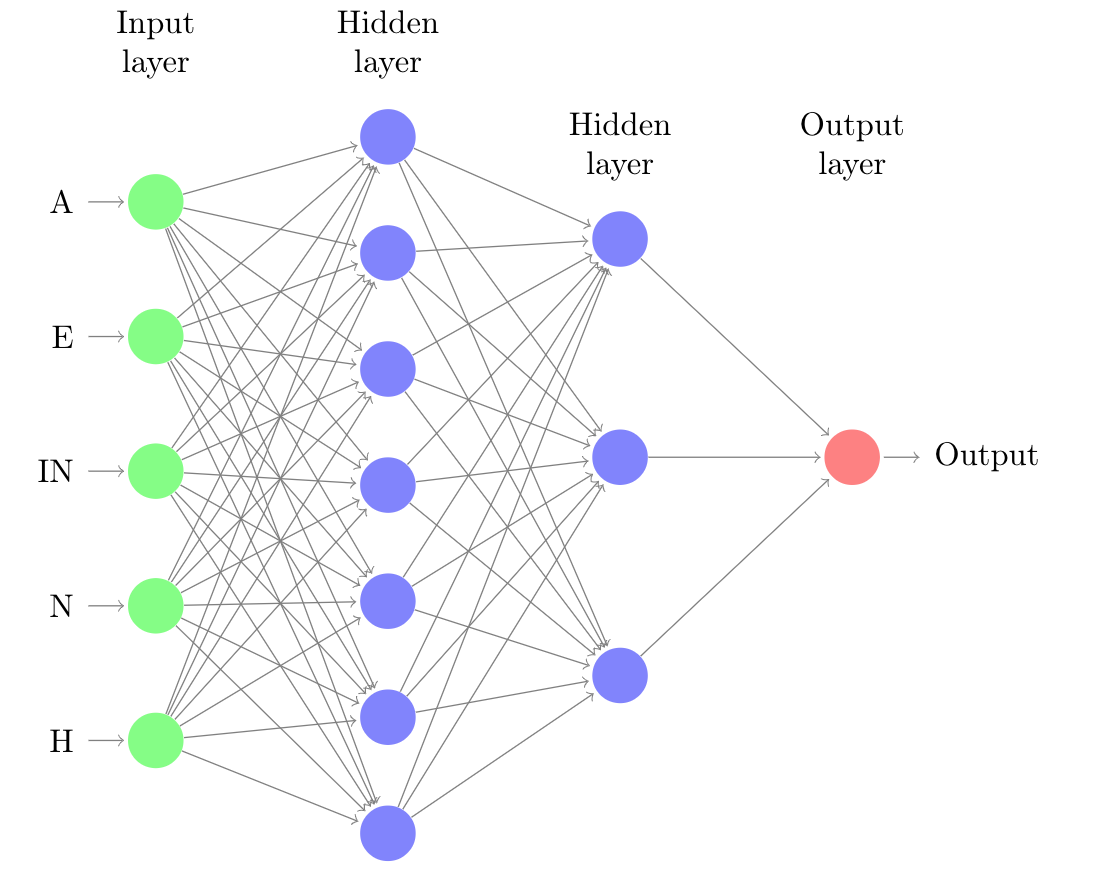
\includegraphics[width=83mm]{images/1_network_hoi.png}
	\centering
	\caption{\label{FIG:HOI_Design} HOI network architecture. The
          input layer (left in green) is comprised of 5 nodes
          representing the input values. The following two layers are
          hidden and comprosed of 7 and 3 nodes, repsectively. The
          final output later is a single node. The tickness of the
          lines connecting the nodes represents the weights in the
          trained network.}
\end{figure}

The input layer is a vector of $5$ neurons to match the dimensionality
of the input, followed by two hidden layers that are composed of 7 and
3 neurons respectively from the input layer. The output is a single
neuron whose values are restrained between 0 and 1 by virtue of the
sigmoid function where objects with a rating of 0.5 or above are
classified as PI and those below the threshold are classified as UO.

The neural-network architecture was arrived at by experimentation.
The network required suffiicent degrees of freedom to properly
generalize the orbital elemental profiles of KI, but without so many
degrees of freedom that overfitting to the training datasets would
pose a problem.

The described architecture, see fig.\,\ref{FIG:HOI_Design} has 69 free
parameters, including 59 weights and 10 biases \footnote{Following the
  architecture described, the number of free parameters can be
  calculated as follows: the input is fed through layers which are
  comprised of 7, 3, and 1 neuron(s). This results in
  5$\times$7+7$\times$3+3$\times$1 weights and 7+3 biases, as only the
  hidden layers have bias parameters.}. To optimize these parameters,
the network is trained on 5 randomly selected sub-sets of $10^5$
observed and $10^5$ KI objects over 28 epochs, which took about 5
minutes on a 3.4\,GHz Intel core-i7 CPU-type. To prevent overfitting,
the training was stopped when the relative loss decrease per epoch
dropped below $1\%$.  At the end of the training process the network's
performance is validate with a subset of 20,000 KI and 20,000 observed
objects that were held out of the training process. Furthermore, all
PHOs are held out of the training process and used exclusively for
testing purposes. Figure \ref{FIG:loss} shows how the loss-function
decreases while the fraction of hazardous objects identified
increases.

\begin{figure}[t]
	\hspace*{-0.3cm}
 	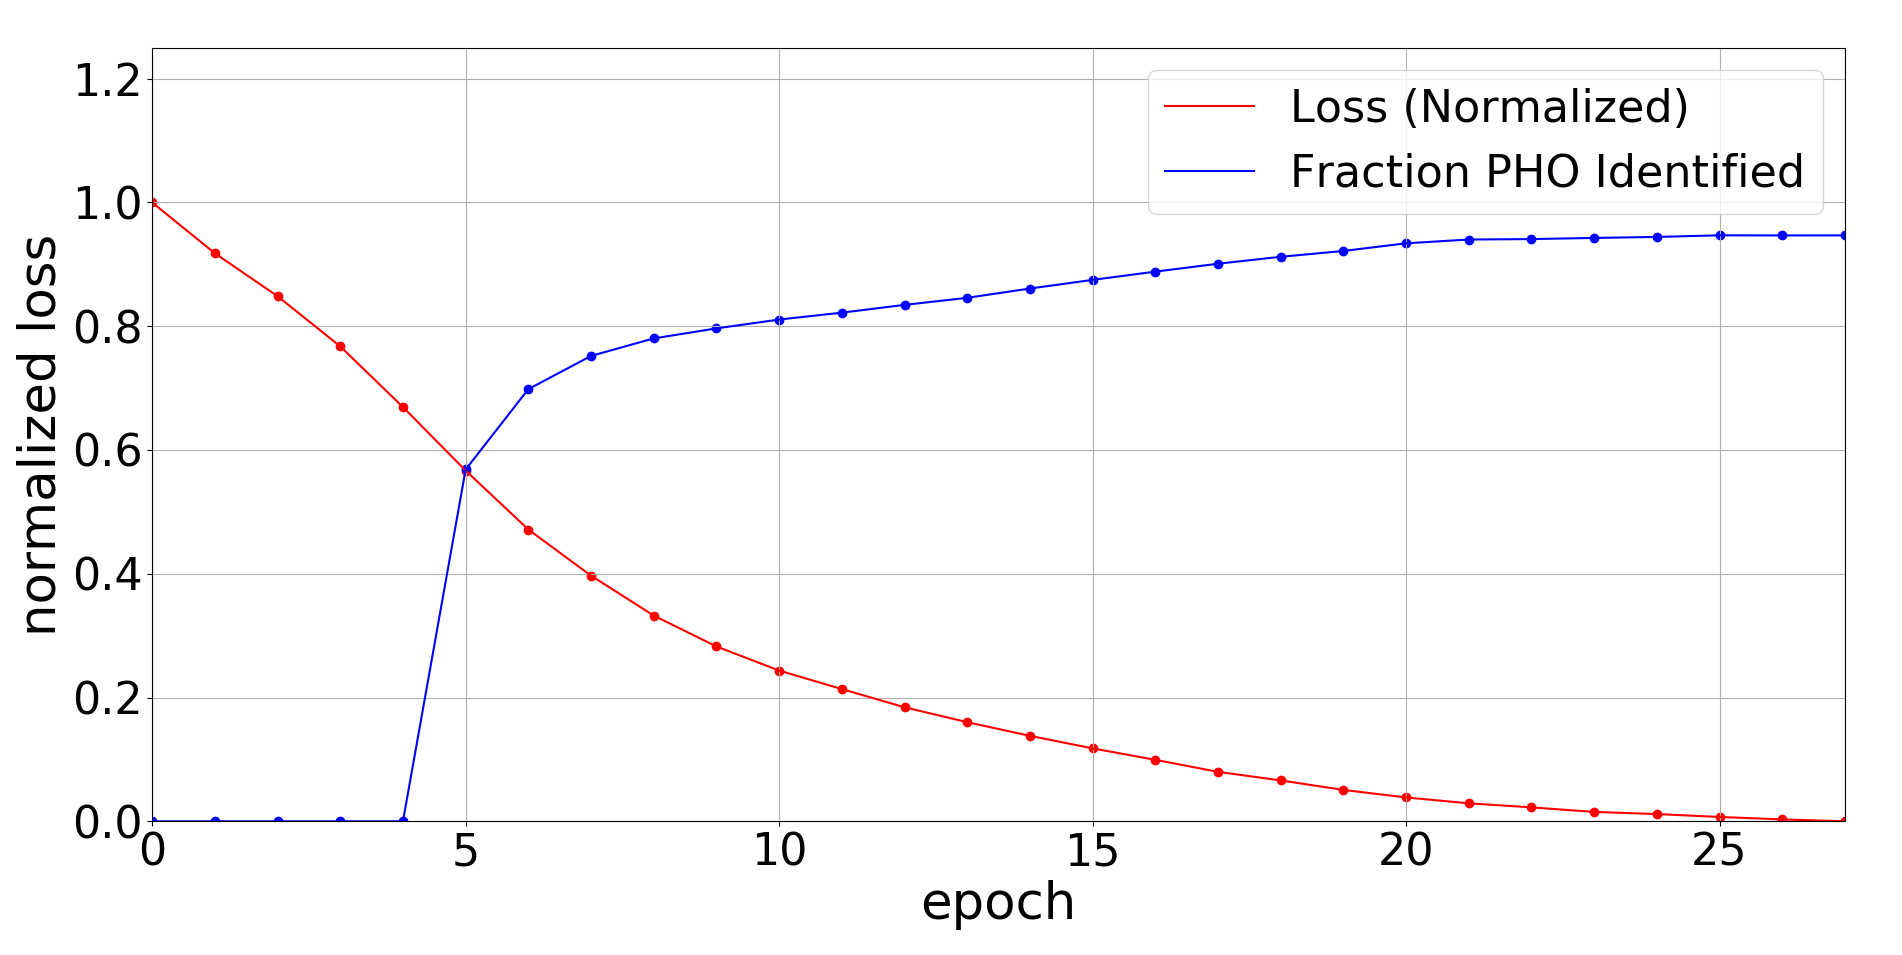
\includegraphics[width=83mm]{images/cost_epoch_pho.png}
	\centering
	\caption{\label{FIG:loss} The normalized loss and fraction of
          identified PHOs as a function of training epoch.}
\end{figure}

Before training, the observed objects and KIs were labeled with 0.1
and 0.9 respectively. Here, higher numbers correspond with a larger
probability of colliding with Earth, meaning that the observed objects
as a whole are assumed to have negligible impact probability.  The
labels are chosen as such to represent the fact that we are not
certain that all the observed objects will not impact Earth and that
the calculation of the KI trajectories are ware not converged
solutions \cite{2014ApJ...785L...3P} and several perturbing effects in
the Solar system ware neglected, so that it cannot be guaranteed that
these objects will collide with Earth when their velocities are
reversed.

Initially, we assumed all individual observed object to be benign.
This seems a safe assumption, because the majority (98.4\%) of the
observed objects used for our experiments have a diameter larger than
100 meter\footnote{ Assuming an absolute magnitude of at most 22.5,
  see Eq. \ref{HtoDiameter} for an albedo of 0.15.}, and those are
expected to impact the Earth less than once every 500 years
\citep{Bostrom}.  We can now estimate an upper-bound of the number of
expected Earth impacts from asteroids in our sample within the next
20,000 years:
\begin{equation}
    N_{collisions}=\int^{\infty}_{100}\frac{4\times10^7}{D^3}=2000.
\end{equation}
Here $D$ is the diameter of an asteroid.  We here ignorded the fact
that many of the existing asteroids have not yet been found.  In
addition, all of the PHOs, which have considerably larger probability
to collide than the rest of the observed population, are not used in
HOI's training and are therefore not mislabeled. We estimate that at
most 0.3\% of the observed objects are mislabeled as
non-impactors. Although our sample contains only a small fraction of
mis-classified non-impactors, they still may affect the performance of
HOI to identify an impactor.

\section{Data generation and acquisition}
\label{SEC:Data}

\subsection{Observed objects}

We extracted $736,496$ minor bodies from NASA's \textit{dastcom5}
database \citep{dastcom5}. About 95.5\% of the extracted objects are
main-belt asteroids, $\sim 3.2$\% are asteroids that are not in the
main belt (such as Apollo or Trojan asteroids), 0.7\% are comets,
0.2\% are Kuiper-belt objects, and the remaining 0.4\% is composed of
a plethora of miscellaneous objects such as planetary satellites and
centaurs \citep{SolarSystemObjects}.  These proportions are probably
not representative of the actual small-body populations because there
is considerable observational bias towards the closer main-belt
asteroids in comparison with more distant objects
\citep{KBO_Population}.

\subsection{Generating a database of known impactors}

We generate a database of KIs as follows.  First we integrate the
Solar system forwards in time for 20,000 years. We now start the
backwards integration. We randomly select 800,000 moments in time at
which we launch KI radially from the Earths' surface with a random
velocity between 11.2 (Earth's escape speed) and 42.5\,km/s (the Solar
system's escape speed), and integrate it backwards in time to the year
2320 together with the rest of the Solar system and the already
orbiting KIs.  We deliberately did not attempt to mimic the observed
asteroid impact velocities to allow the neural network to learn from
the full range of parameters rather than on a hand-selected subsample.

We did not consider asteroids that would impact the Earth in the
coming 300 years \footnote{An object, for example, that is launched
  from the solar system at the year 2320, and is then integrated
  backwards in time 300 years, would create an example of a present
  day asteroid that would strike the Earth in 300 years after the
  velocity vectors are negated to account for time reversal.}. In this
way we generate a database of 470,000 KIs that orbit the Sun in the
year 2020, and of which we know it will impact Earth some time in the
next 20,000 years. This number is smaller than the inital anticipated
800,000 because objects either left the Solar system, were unable to
escape Earth's gravitational field, or spun into the Sun.

\section{Results}
\label{SEC:Results}

\subsection{Identifying impacting asteroids}

The training of the network leads to the positive identification of
95.25\% of KIs that ware not part of the training.  From objects that
are indicated by NASA as PHOs the network indentifies 90.99\%, and
1.94\% as PIs.  The high fraction correctly identified KIs indicates
that HOI positively recognizes nearly every object that is constructed
to strike Earth.  This performance is not unexpected because HOI was
specifically tuned to identify artificial KI objects. A more
meaningful metric of performance is the percentage of PHOs
identified. Although 9.01\% PHOs were not classified as potential
impactors, HOI is approximately 47 (90.99/1.94) times more likely to
select a PHO over some other observed object.  We classify a total of
14,680 out of $736,496$ asteroids as potentially hazardous.

To further evaluate the effectiveness of HOI, we performed simulations
to compare the closest approaches of PIs to UOs relative to Earth. The
algorithm utilized to perform these calculations is the same in every
respect to the algorithm with the exception that each object is
integrated forward in time for 1,000 years. The trajectories of 14,680
identified PIs and an equal amount of randomly selected observed
asteroids are computed. In figure \ref{FIG:Closeness_Histogram}, we
present the distribution of closest approaches reached during these
integrations.

\begin{figure}[h]
	\hspace*{-0.35cm}
	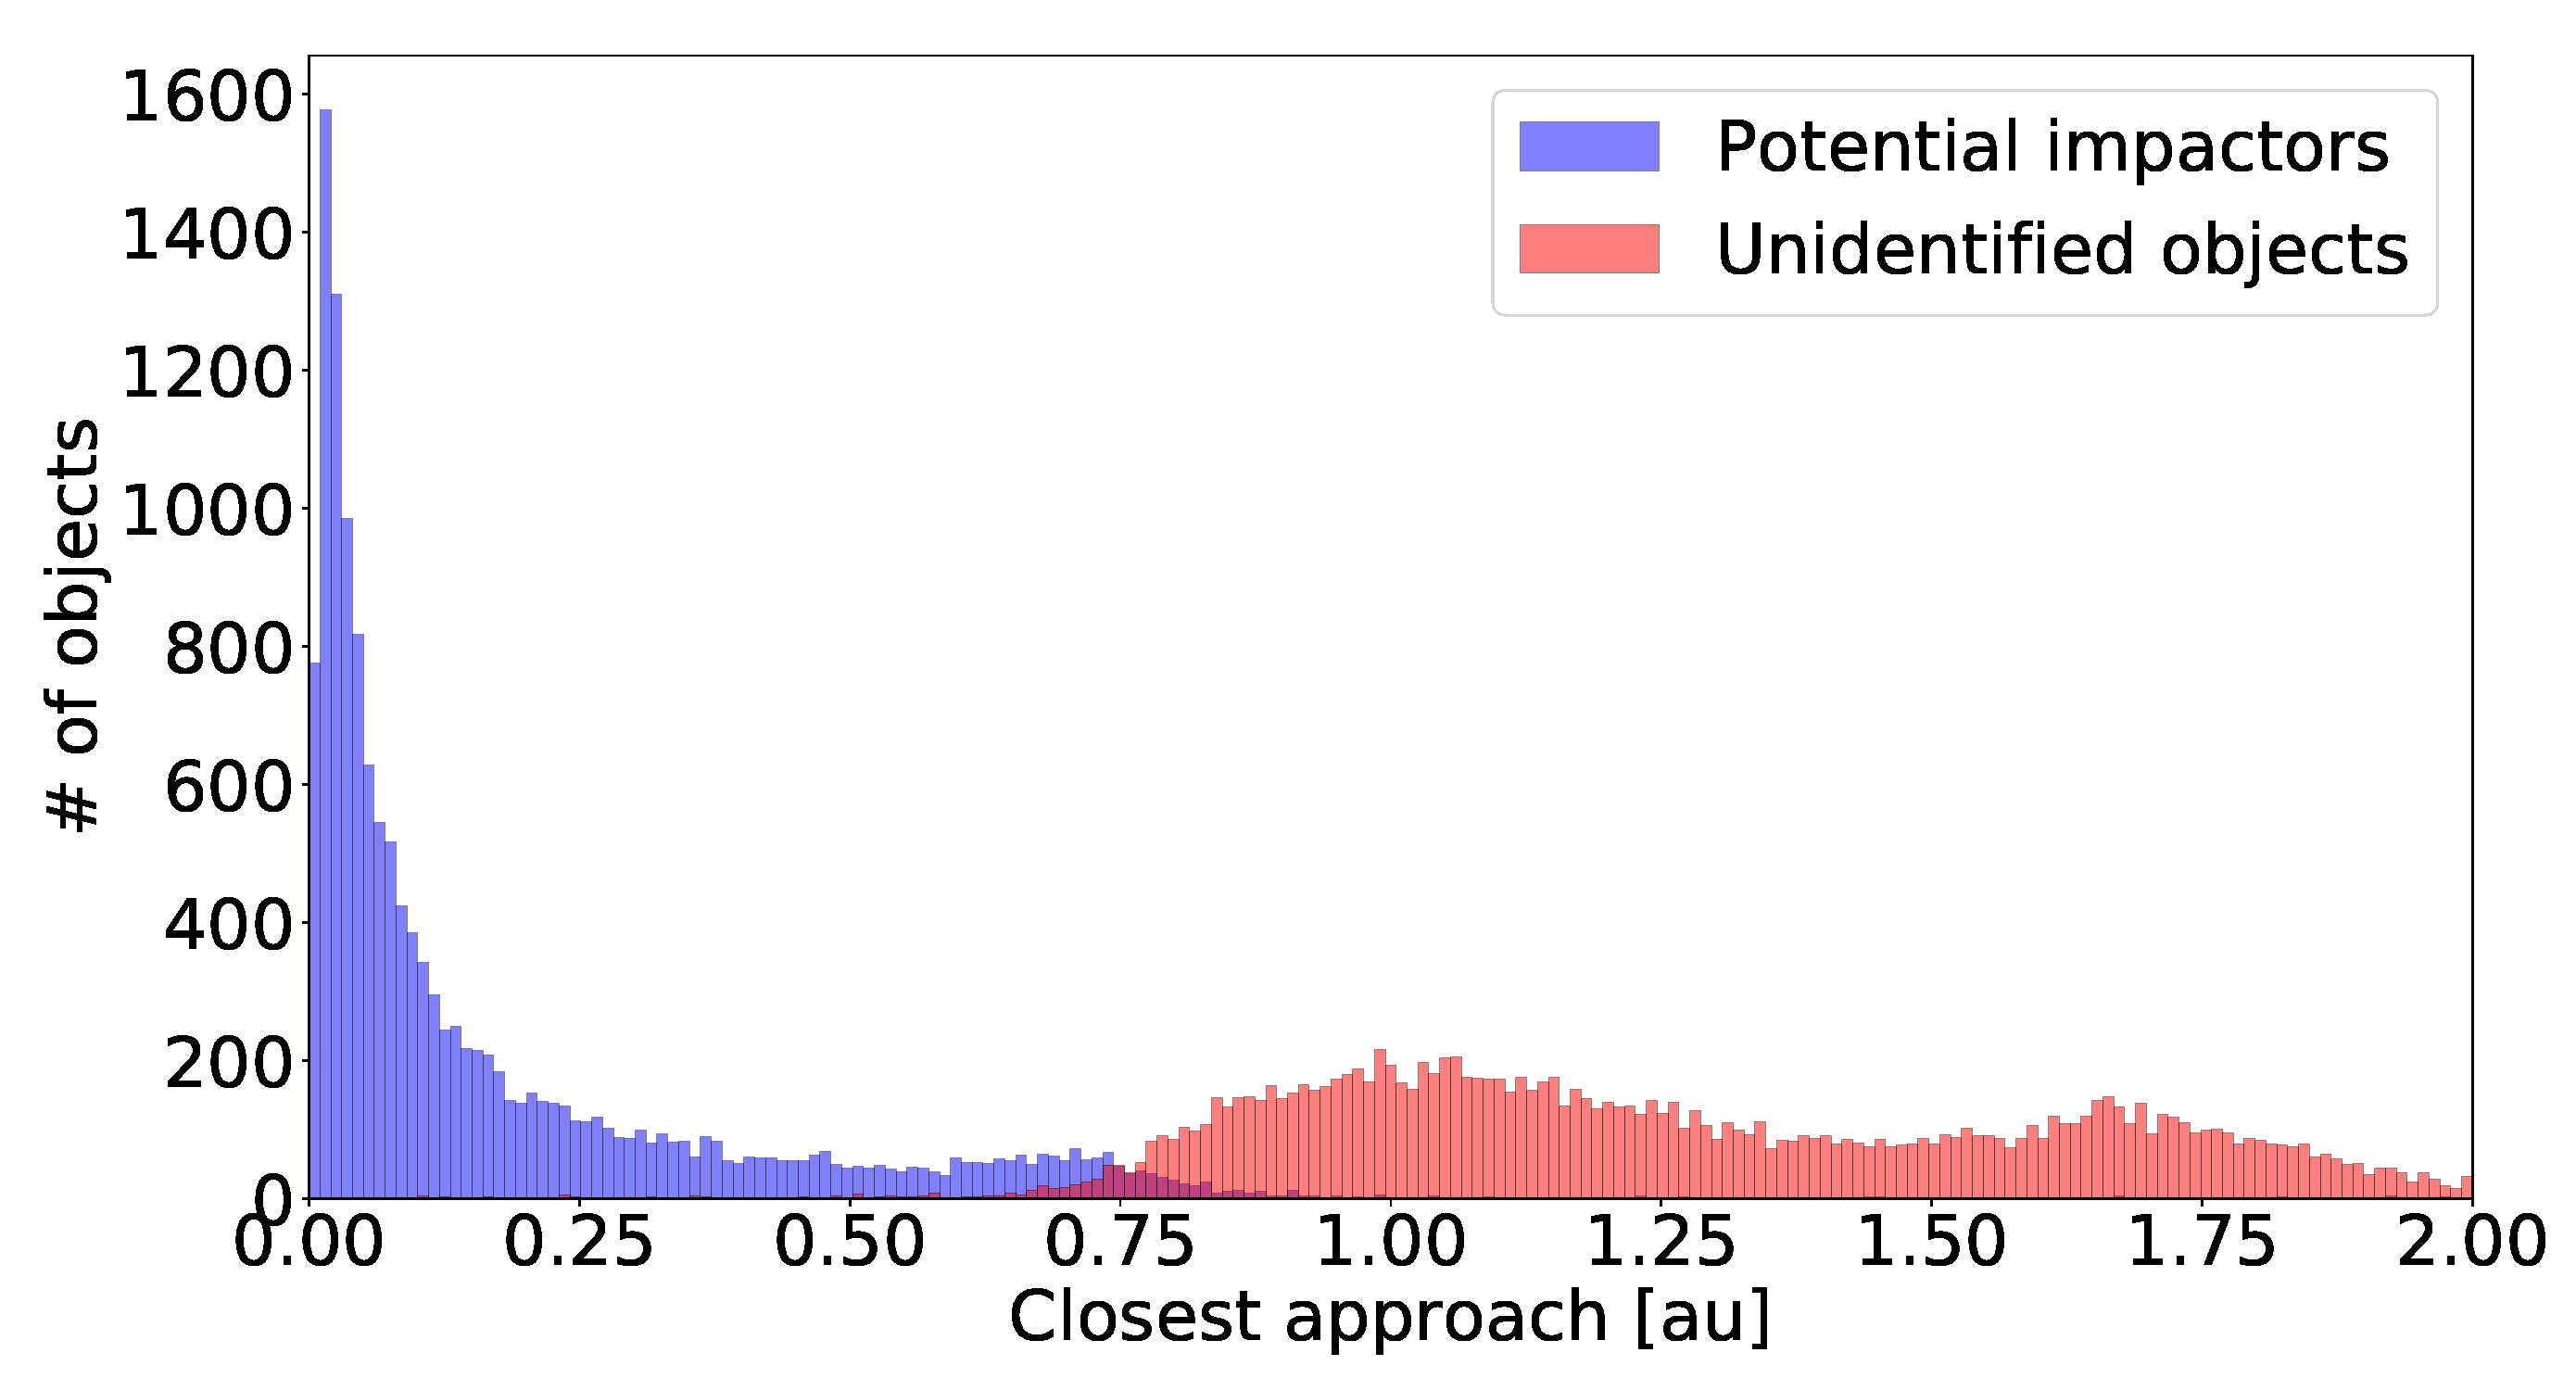
\includegraphics[width=83mm]{images/3_Closest_Approach_Together.pdf}
	\centering
	\caption{\label{FIG:Closeness_Histogram} The closest distance
          from Earth in the next 1000 years from objects classified by
          HOI as potentially hazardous.  We took out 108 PIs and 884
          unselected observed objects, because their closest
          approaches exceeded the x-axis limits of 2 \,au. Virtually
          every object that reach Earth within 0.01\,au and 99.9\% of
          objects within 0.05\,au are identified by HOI as PIs.
}
\end{figure}
 
To investigate why HOI only identifies approximately nine-tenths of
PHOs as PIs, the thousand-year integrations described above performed
for all unidentified PHOs. We present in Fig.\,
\ref{FIG:Closeness_PHOs} the probability density function of these
closest approaches.  The distributions of identified PHOs and
unidentified PHOs are similar, and the fraction of objects identified
as PHOs or PIs could be used as a measure of the network's
performance.  In addition, all objects that did not approach Earth
within at least 0.5\,au could be considered misclassified PIs. This
cut-off is not arbitrary, but is rather based on the minimum distance
achieved by 99.7 percent, or $2\sigma$, of PHOs. In the case of HOI,
12.2\% of the PIs are outside of this threshold and are therefore
considered misclassified. The root of this misclassification stems
from the fact that not all of the KIs collide with Earth when
integrated forward in time for only 1000 years, and that all of the
observed objects are a-priori not benign. This implies that the
labeling scheme used to train HOI is not perfect.  \simon{How can we
  improve this naming scheme?}

\begin{figure}[h]
    \hspace*{-0.44cm}
	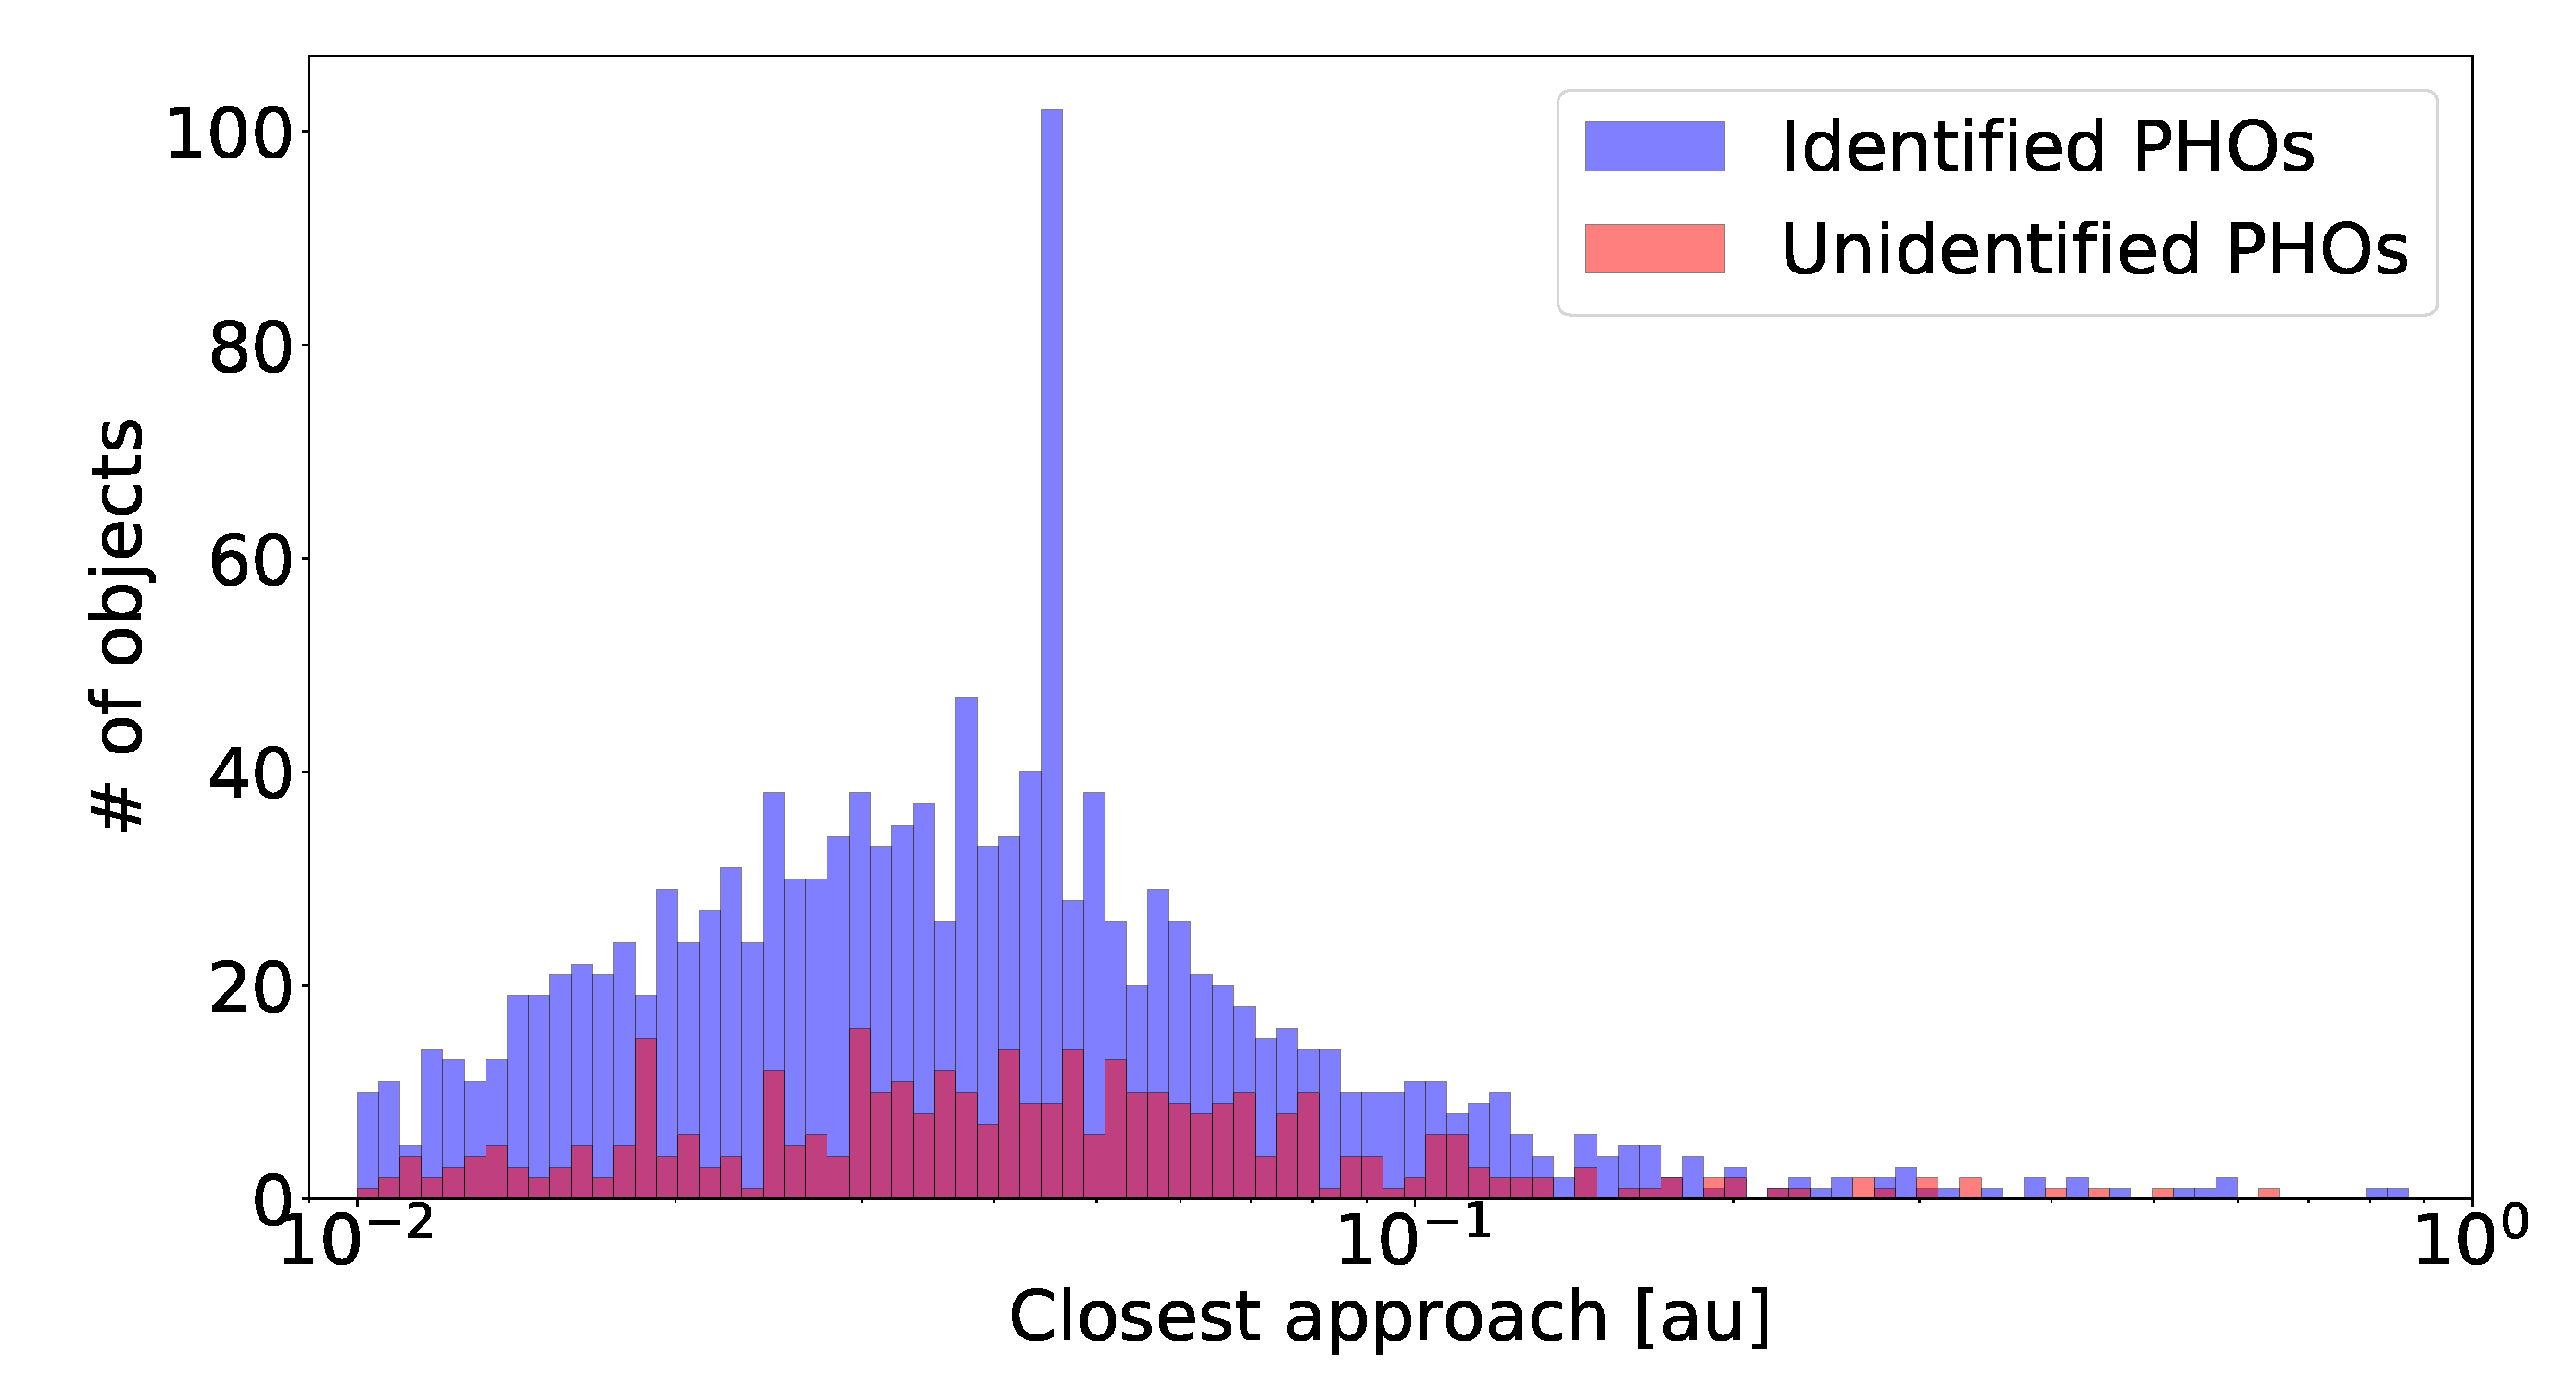
\includegraphics[width=85mm]{images/4_Closeness_Plots_PHOsLog.pdf}
	\centering
	\caption{\label{FIG:Closeness_PHOs} Te closest approach
          distance to Earth reached for positively identified objects
          by HOI in the coming 1000 year.
          \simon{Linear scale in
            $x$.}}
\end{figure}

A total of $13,258$ asterids identified by HOI as KIs are not lised by
NASA as PHO.  In our thousand-year integrations, $4472$ of these
approach to within 0.05\,au of Earth while $2015$ will approach to
within 0.02\,au.  In Table.\,\ref{TAB:Short_List} we present a short
list of the 11 most hazardous asteroids with absolute magnitudes of
less than 22 and data arcs of less than 31 days.

\begin{table}[]
\begin{tabular}{lcrlr}
\hline \hline
\bf{Designation} & \bf{CA} & \bf{$t_{\rm CA}$} & \bf{H} & \bf{arc} \\
                 & [au]    & [Year] & [mag] & [day] \\
\hline 
2005 RV24 & 0.020 &  Feb. 2374 & 20.60 & 28 \\
2008 UV99 & 0.013 &  April 2332 & 20.03 & 1 \\
2011 BU10 & 0.006 &  April 2920 & 21.30 & 18 \\ 
2011 HH1 & 0.012 &  July 2923 & 21.7 & 13 \\ 
2011 WC44 & 0.018 & Feb. 2679 & 20.5 & 31 \\ 
2013 AG76 & 0.013 &  Dec. 2638 & 20.3 & 24 \\ 
2014 GL35 & 0.018 & July 2556 & 20.6 & 23 \\ 
2014 TW57 & 0.017 & Sept. 2165 & 20.1 & 24 \\ 
2014 WD365 & 0.017 & Sept. 2735 & 19.7 & 5 \\
2017 DQ36 & 0.013 &  Dec. 2131 & 19.3 & 29 \\ 
2017 JE3 & 0.016 & July 2741 & 21.9 & 23 \\
\hline \hline
\vspace{0.5cm}
\end{tabular}
\caption{\label{TAB:Short_List} Short list of relatively large minor
  bodies with a short data arc that ware identified as potentially
  hazardous by HOI and which are not in NASA's \textit{dastcom5}
  database \citep{dastcom5}.  along with their closest approach (CA)
  in au, the month and year that their closest approach occurred
  ($t_{\rm CA}$), their absolute magnitude (H), and their data arc
  length in days (arc).}
\end{table}

The absolute magnitude threshold of $22$ is chosen so that only
asteroids that have the potential of causing regional devastation
unprecedented in human history make the short-list.  With a geometric
albedo between $0.05$ and $0.25$ objects with an absolute magnitude of
$22$ have a diameter from $\sim 100$\,m to $236$\,m. Even a small
diameter object would be comparable in size to the body that produced
the Tunguska crater, flattening $2,000$ square kilometers of forest in
Siberia \citep{Tunguska}.
 
The month-long data-arc limit is selected because the Monte-Carlo
method adopted by NASA is particularly ill-suited for calculating the
impact probabilities of such uncertain orbits.  As a consequence,
these objects are the most likely to be overlooked as potential
impactors. Since each came within 0.02\,au of Earth during our
thousand-year integrations, we consider them potentially dangerous.

\subsection{Comparing various populations of object}

The characteristics of simulated KI and the observed populations are
compared to better understand how HOI differentiates between the two
populations. In figure \ref{FIG:Object_Trajectories} we present 100
trajectories of observed objects and KIs.

\begin{figure*}[h!]
    \hspace*{-0.40cm}
	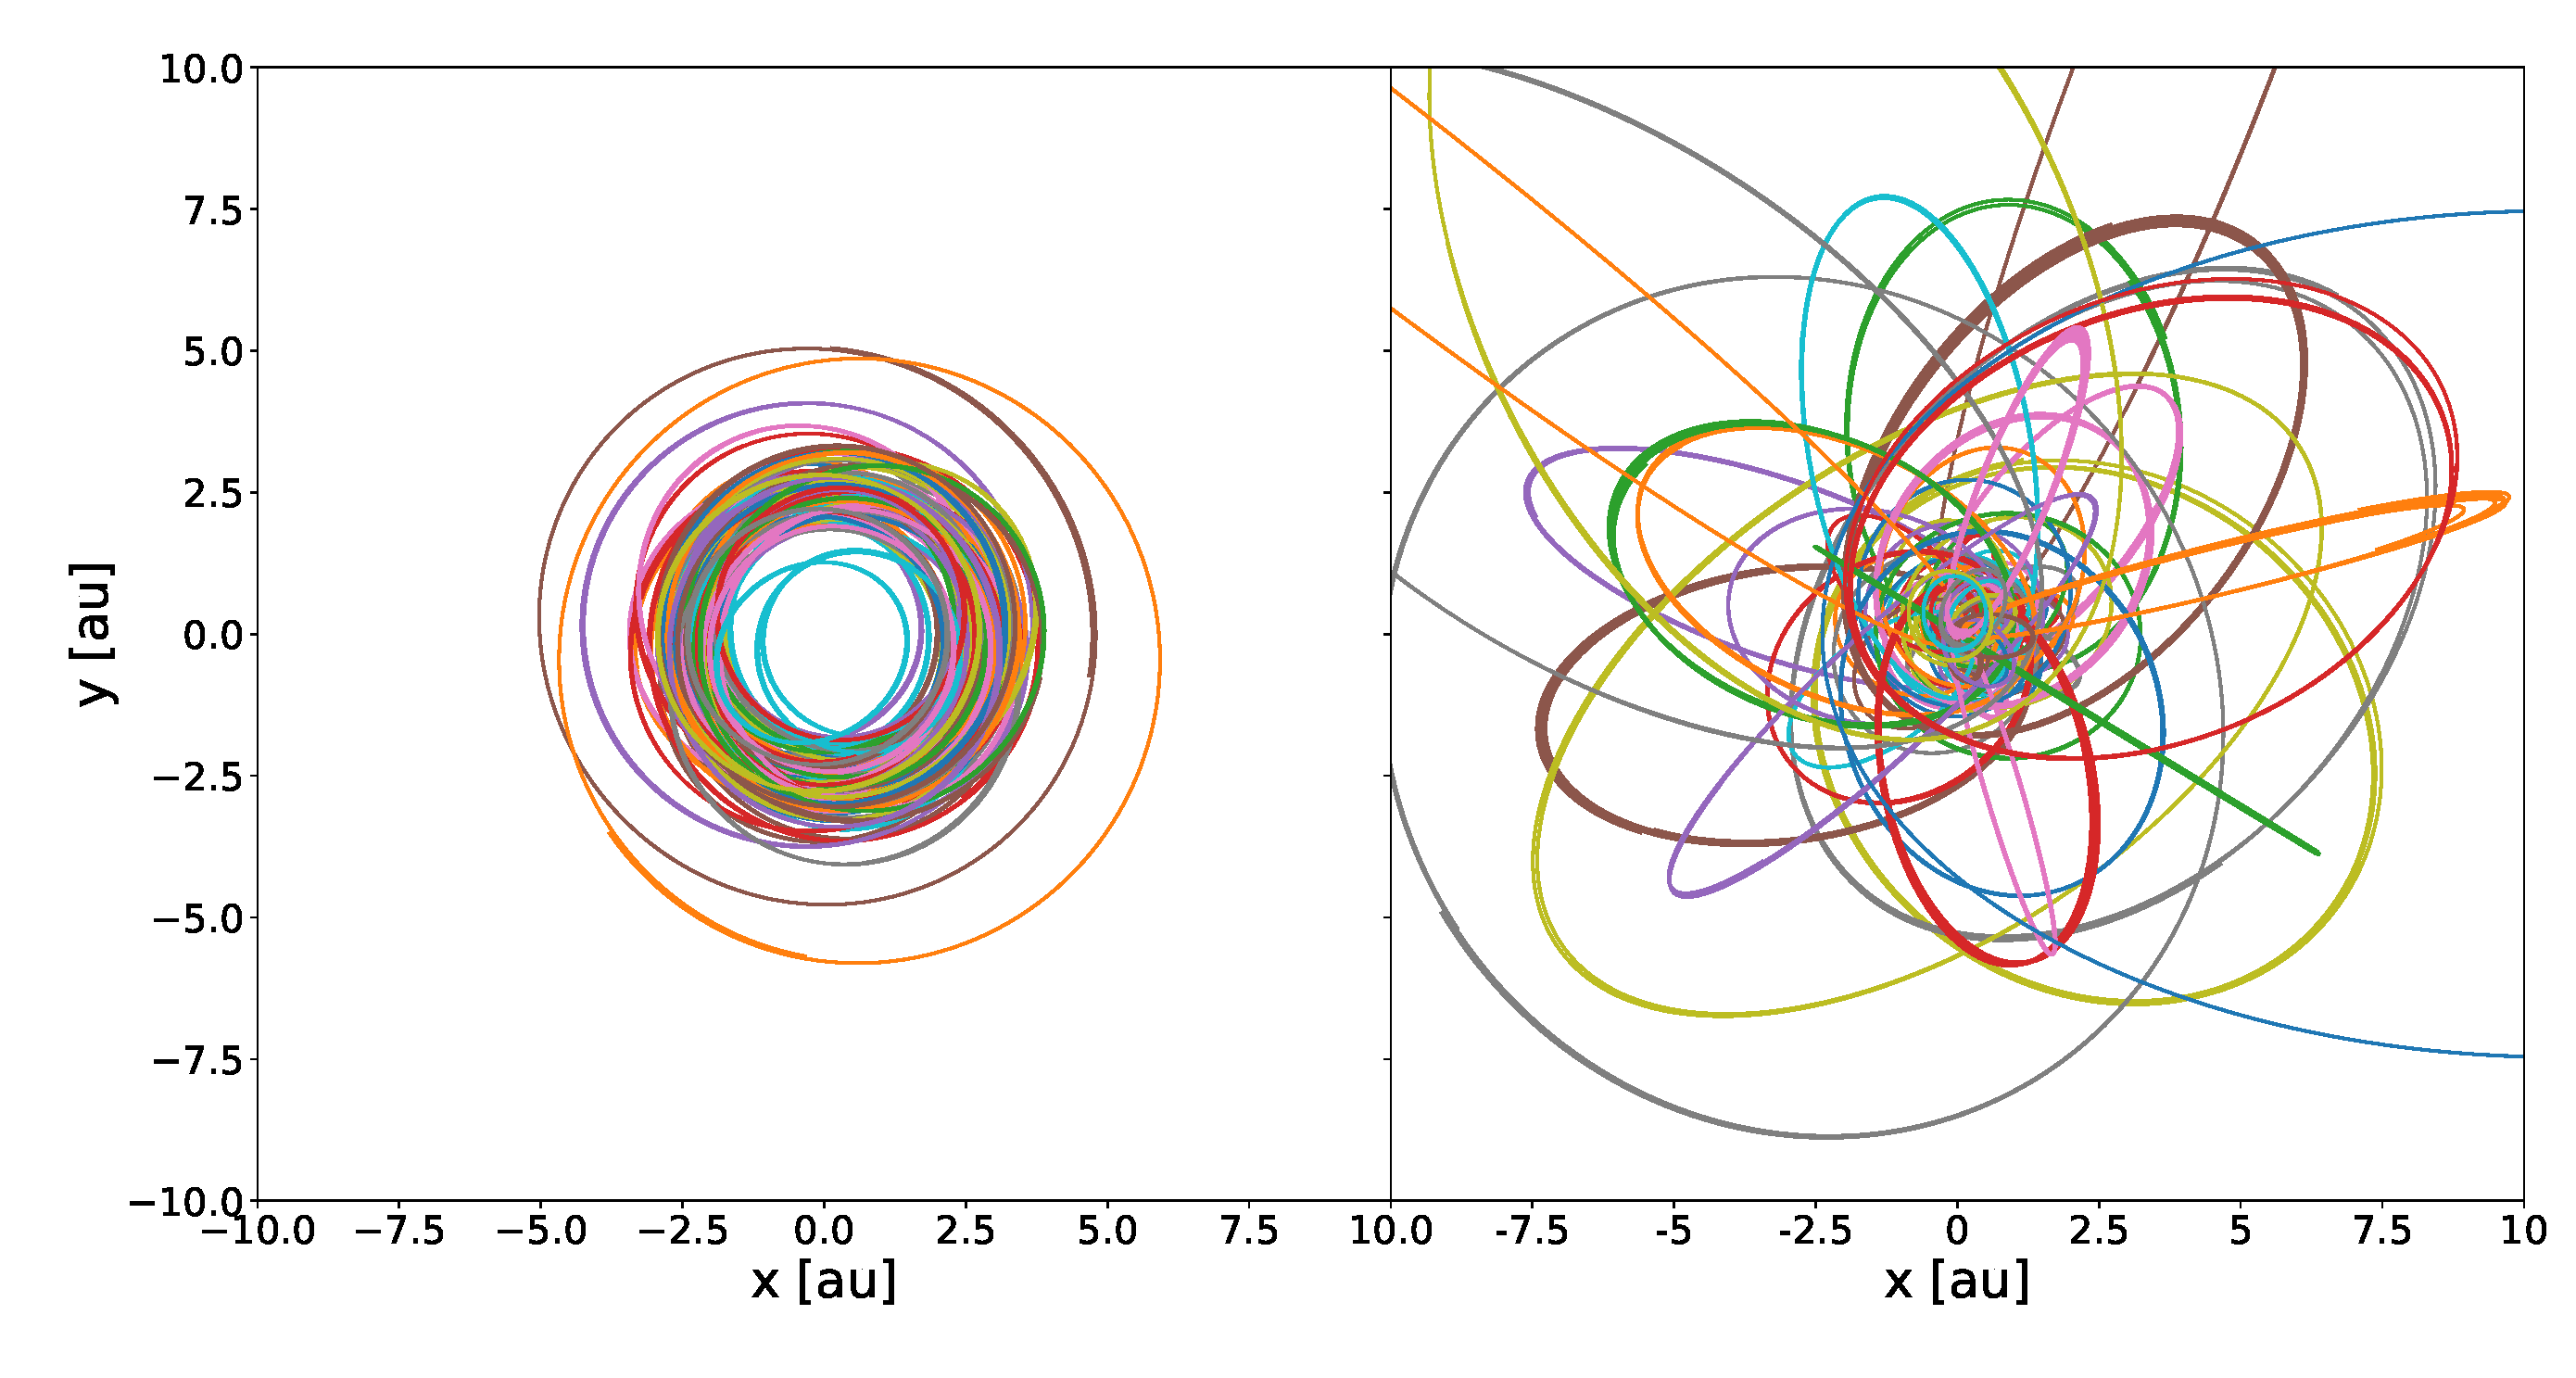
\includegraphics[width=170mm]{images/5_Trajectories.pdf}
	\centering
	\caption{\label{FIG:Object_Trajectories} Illustration of the
          difference between the trajectories of observed objects
          (left) and known-impactors as we generated them to train HOI
          (right). The observed objects tend to have circular orbits
          which in the orbital plane of Earth around the Sun, whereas
          the known-impactors exhibit a much broader distribution in
          eccentricity and inclination. These characterics, however,
          are not mutually exclusive and could be one the root causes
          of HOI's imperfect classification.}
\end{figure*}

There are profound differences between the orbital elements of the two
distinct populations of objects. Our artificial population of objects
launched from Earth tend to have highly eccentric and inclined orbits,
whereas the observed objects tend to have circular orbits confined
near the ecliptic plane. For the observed objects, the orbital plane
is essentially empty within approximately 2\,au of the Sun, while for
the KIs this is the most densely occupied space. This object
distribution, however, should be expected considering that the all KIs
were generated $1\pm0.017$\,au away from the Sun along the Earth's
orbit. During the short time-scale integration it is not expected that
these objects migrate to widely different orbits.

\section{Conclusions}
\label{SEC:Conclusions}

We designed, constructed and trained a rather simple neural network to
classify asteroids as potentially impacting Earth in the coming
$20,000$ years. Our method takes the observed orbital elements as
input and provide a classifier for the expectation value of the object
striking Earth.

The network was able pick out 95.25\% of the known impactors (KIs)
when mixed into a set of observed asteroids which are not expected to
strike Earth. When applied to the entire population of observed
asteroids, the network was able to identify nearly nine-tenths of the
asteroids identified by NASA as potentially hazardous and virtually
every asteroid that approached within 0.05\,au of Earth.  We generate
a short list of network identified potential impacting asteroids which
NASA does not label potentially hazardous, mainly because the observed
orbital elements are so uncertain that NASA's Monte Carlo approach to
determine their Earth-striking probability fails.

The network classifies an object as a potential impactor within $0.25$
milliseconds, which is negligible compared to the time required for
the Monte-Carlo method employed by NASA.
 
Follow-up calculations over a time-span of 1000 years reveals that
12.2\% of the potential impactors identified in the network, did not
come within 0.5\,au of Earth. This may imply that they asteroids pose
no direct threat on the time scale considered. Integrating their
orbits for a longer time-frame, however, is unpractical because of the
large uncertainty in their orbital elements and the relatively small
Lyapunov time scale for these obejcts.

We envison to improve the network's classification accuracy.  The
network, as we present in in fig.\,\ref{FIG:HOI_Design}, is the result
of much experimentation in network depth, width and (sub)selecting
input parameters. Maybe that structure preserving mimetic
architectures motivated by the underlying Keplerian topology of the
orbits allow us to achieve a higher predicting quality, but this still
requires considerable experimentation.  Another improvement could be
realized by considering a stricter labeling scheme in which some
probability statistics on striking the Earth could be taken into
account.

\begin{acknowledgements}
  
  We thank the Microsoft Cooperation for access to the Azure cloud on
  which many of the calculations presented here are performed.  JDH
  thanks Sander van den Hoven for his mentoring during an internship
  at Microsoft Amsterdam. This work was supported by the Netherlands
  Research School for Astronomy (NOVA), NWO (grant \# 621.016.701
  [LGM-II]).

\end{acknowledgements}
\bibliographystyle{aa}
\bibliography{bibliography}

\end{document}


